
\chapter{Preliminaries}
\label{cha:preliminaries}

In this chapter, we will introduce the preliminaries which are necessary for the rest of the thesis.
In Section~\ref{sec:prelim-dls}, we introduce \emph{description logics (DLs)} as a well-established
logical formalism for knowledge representation and show the specific notations used in this thesis
to emphasise parameters which are important later on. A short overview of the ontological
foundations of roles followed by the presentation of the formal role-based modelling language CROM
is given in Section~\ref{sec:role-based-modelling}.

\section{Description Logics}
\label{sec:prelim-dls}

Description logics are a family of knowledge representation formalisms. As already outlined in the
introduction, DLs allow to represent application domains in a well-structured way. In this section,
we present the notations, definitions and known results which are used in this thesis.
%
For a more thorough introduction into description logics we refer the reader to
\cite{DLhandbook-07}.

\subsection{Description Logic Concepts}
\label{sec:dl-concepts}

As shown in Section~\ref{sec:intro-description-logics}, DL concepts describe sets of
elements. Concepts are build from \emph{concept names}, \emph{role names} and \emph{individual
  names} using concept and role constructors.  Note that in the following definitions we refer to
the triple $\Nsig \coloneqq (\NC, \NR, \NI)$ explicitly although it is usually left implicit in
standard definitions.  This turns out to be useful in Chapter~\ref{cha:context-dls} as we need to
distinguish between different DLs and symbols used in the meta level and the object level.
Sometimes we omit \Nsig, however, if they are irrelevant or clear from the context.

\begin{definition}[Syntax of roles over \Nsig and concepts over \Nsig]
  \label{def:syntax-concepts}
  Let~\NC, \NR, \NI be countably infinite, pairwise disjoint sets of
  \emph{concept names}, \emph{role names}, and \emph{individual names}. Then, the triple
  $\Nsig\coloneqq(\NC,\NR,\NI)$ is a \emph{signature}. A \emph{role $r$ over \Nsig} is either
  a role name, i.e.~$r\in\NR$, or it is of the form $s^{-}$ with $s\in\NR$ (\emph{inverse role}).

  The set of \emph{concepts over \Nsig} is the smallest set such that
  \begin{itemize}
  \item for all $A\in\NC$, then $A$ is a concept over \Nsig (\emph{atomic concept}), and
  \item if $C$ and $D$ are concepts over \Nsig, $r$ is a role over \Nsig and $a\in\NI$, then
    $\lnot C$ (\emph{negation}), $C\sqcap D$ (\emph{conjunction}), $\exists r.C$ (\emph{existential
      restriction}), $\{a\}$ (\emph{nominal}) and $\atleast{n}{r}{C}$ (\emph{at-least restriction})
    are concepts over \Nsig. \qedhere
  \end{itemize}
\end{definition}

\noindent Non-atomic concepts are also called \emph{complex concepts}. As usual in description
logics, we use the following abbreviations:
\begin{itemize}
\item $C\sqcup D$ (\emph{disjunction}) for $\lnot(\lnot C \sqcap \lnot D)$,
\item $\top$ (\emph{top}) for $A \sqcup \lnot A$ where $A\in\NC$ is arbitrary but fixed,
\item $\bot$ (\emph{bottom}) for $\lnot\top$,
\item $\forall r.C$ (\emph{value restriction}) for $\lnot(\exists r.\lnot C)$, and
\item $\atmost{n}{r}{C}$ (\emph{at-most restriction}) for $\lnot(\atleast{n+1}{r}{C})$.
\end{itemize}

\noindent
The semantics of description logic concepts are defined in a model-theoretic way using the notion of
interpretations.

\begin{definition}[\Nsig-interpretation, Semantics of concepts over \Nsig]
  \label{def:n-interpretation}
  Let $\Nsig\coloneqq(\NC,\NR,\NI)$ be the signature. Then, an \emph{\Nsig-interpretation \I} is a pair
  $(\Delta^{\I}, \cdot^{\I})$ where the \emph{domain} $\Delta^{\I}$ is a non-empty set and
  the \emph{interpretation function} $\cdot^{\I}$ maps
  \begin{itemize}
  \item every concept name $A\in\NC$ to a set $A^{\I}\subseteq\Delta^{\I}$,
  \item every role name $r\in\NR$ to a binary relation
    $r^{\I}\subseteq\Delta^{\I}\times\Delta^{\I}$, and
  \item every individual name $a\in\NI$ to an element $a^{\I}\in\Delta^{\I}$ such that different
    individual names are mapped to different elements, i.e.\ for $a,b\in\NI$ it holds that
    $a^{\I}\neq b^{\I}$ if $a\neq b$.
  \end{itemize}
  %
  This function is extended to inverse roles and complex concepts as follows:
  \begin{itemize}
  \item $(s^{-})^{\I} \coloneqq \left\{(d,c)\in\Delta^{\I}\times\Delta^{\I}\mmid (c,d)\in
      s^{-}\right\}$,
  \item $(\lnot C)^{\I} \coloneqq \Delta^{\I} \setminus C^{\I}$,
  \item $(C \sqcap D)^{\I} \coloneqq C^{\I} \cap D^{\I}$,
  \item $(\exists r.C)^{\I} \coloneqq \{d \in \Delta^\I \mid \text{there is an}\ e \in C^\I \
    \text{with}\ (d,e)\in r^\I\}$,
  \item $\{a\}^{\I} \coloneqq \{a^{\I}\}$, and
  \item $(\atleast{n}{r}{C})^{\I} \coloneqq \{d \in \Delta^{\I} \mid \sharp\{e\in C^{\I}\mid (d,e)\in r^{\I}\}\ge n\}$.
  \end{itemize}
  where $\sharp S$ denotes the cardinality of the set $S$.
\end{definition}

\noindent
For any $x\in\NC\cup\NR\cup\NI$, $x^{\I}$ is called the \emph{extension of $x$}.  Note that in the
above definition of an interpretation, we adopt the so-called \emph{unique name assumption} stating
that every individual name is interpreted as a distinct element. By doing so, we emphasize that an
individual name is meant to be the identity of an individual, rather than just a tag as it is
usually used in the context of semantic web.

Now, we can look at a first example using the notions just defined.

\begin{example}\label{ex:concept-nfl}
  Consider the following complex concept $C$:
  \begin{align*}
    & \mathsf{NFL\_{}Team} \sqcap \lnot \mathsf{AFC} \sqcap
    \atleast{1}{\mathsf{playsFor}^{-}}{(\exists\mathsf{position}.\mathsf{Quarterback})} \\
    & \qquad\sqcap \exists\mathsf{coaches}^{-}.\{\text{\textit{MikeMcCarthy}}\}
  \end{align*}
  It describes all NFL teams which are not in the AFC, have at least one person playing for them at
  quarterback position and are coached by Mike McCarthy.

  Figure~\ref{fig:example-concept} depicts an interpretation in which the Green Bay Packers are in the extension of the above concept.
\end{example}
\begin{figure}
  \centering
  \begin{tikzpicture}
    \node[node, label={[align=center]180:\textit{GreenBayPackers},\\\textsf{NFL\_Team}, \textsf{NFC}}] (gbp) at (0,0) {};
    \node[node, label={[align=center]270:\textit{MikeMcCarthy}}] (mmc) at (4,1.0) {};
    \node[node, label={[align=center]270:\textit{AaronRodgers}, \\\textsf{NFL\_PLayer}}] (ar) at (4,-1.0) {};
    \node[node, label={[align=center]270:\textsf{Quarterback}}] (qb) at (8,-1.0) {};
    %
    \draw[edge] (mmc) to[bend right=10,swap] node{$\mathsf{coaches}$} (gbp);
    \draw[edge] (ar) to[bend left=10] node{$\mathsf{playsFor}$} (gbp);
    \draw[edge] (ar) to[bend left=10] node{$\mathsf{position}$} (qb);
  \end{tikzpicture}
  \caption{An Interpretation \I such that $\text{\textit{GreenBayPackers}}^{\I} \in C^{\I}$ and
    $\I\models\Omc$ with $C$ from Example~\ref{ex:concept-nfl} and \Omc from Example~\ref{ex:bkb-nfl}.}
  \label{fig:example-concept}
\end{figure}



\subsection{Boolean Knowledge Bases}
\label{sec:dl-axioms}

With the notion of concepts at hand, we can formulate \emph{axioms} to capture domain knowledge in a
so-called \emph{Boolean knowledge base (BKB)}. Each BKB consists of a Boolean combination of certain
axioms and an RBox which states the general knowledge about roles.

\begin{definition}[Syntax of axioms over \Nsig and BKBs over \Nsig]
  Let $\Nsig\coloneqq(\NC,\NR,\NI)$ be the signature. Then, if $C$ and $D$ are concepts over \Nsig, $r$
  and $s$ are roles over \Nsig, and $\{a,b\}\subseteq\NI$, then
  \begin{itemize}[itemsep = 6.0pt plus 2pt minus 1pt, topsep = 11pt plus 3pt minus 5pt]
  \item $C \sqsubseteq D$ (\emph{general concept inclusion, GCI}),
  \item $C(a)$ (\emph{concept assertion}),
  \item $r(a,b)$ (\emph{role assertion}),
  \item $r \sqsubseteq s$ (\emph{role inclusion}), and
  \item $\mathsf{trans}(r)$ (\emph{transitivity axiom})
  \end{itemize}
  are \emph{axioms over \Nsig}.
  %
  Moreover, an \emph{RBox \Rmc over \Nsig} is a finite set of role inclusions over \Nsig and
  transitivity axioms over \Nsig. A \emph{Boolean axiom formula over \Nsig} is defined inductively
  as follows:
  \begin{itemize}[itemsep = 6.0pt plus 2pt minus 1pt, topsep = 11pt plus 3pt minus 5pt]
  \item every GCI over \Nsig is a Boolean axiom formula over \Nsig,
  \item every concept and role assertion over \Nsig is a Boolean axiom formula over \Nsig,
  \item if $\Bmc_{1}$, $\Bmc_{2}$ are Boolean axiom formulas over \Nsig, then so are $\lnot\Bmc_{1}$
    (axiom negation) and $\Bmc_{1}\land\Bmc_{2}$ (axiom conjunction), and
  \item nothing else is a Boolean axiom formula over \Nsig.
  \end{itemize}
  %
  Finally, a \emph{Boolean knowledge base (BKB) over \Nsig} is a pair
  $\Bmf = (\Bmc, \Rmc)$, where \Bmc is a Boolean axiom formula over \Nsig and \Rmc is an
  RBox over \Nsig. An \emph{ontology over \Nsig} is an BKB over \Nsig, where only
  axiom conjunction and no axiom negation is allowed in the Boolean axiom formula.
\end{definition}

\noindent
Again as usual in description logics, we use $C \equiv D$ (\emph{concept equivalence}) as abbreviation
for $(C \sqsubseteq D) \land (D \sqsubseteq C)$ and $\Bmc_1\lor\Bmc_2$ (\emph{axiom disjunction}) as
abbreviation for $\lnot(\lnot\Bmc_1\land\lnot\Bmc_2)$.
%
Often an ontology $\Omc = (\Bmc, \Rmc)$ is written as a triple $\Omc = (\Tmc, \Amc, \Rmc)$ where
\Tmc (\emph{TBox}) is the set of all GCIs occurring in \Bmc and \Amc (\emph{ABox}) is the set of all
assertion axioms occurring in \Bmc.


\begin{definition}[Semantics of axioms over \Nsig, BKBs over \Nsig]
  \label{def:semantics-of-axioms}
  An \Nsig-interpretation \I is a model of
  \begin{itemize}
  \item the GCI $C \sqsubseteq D$ over \Nsig if $C^{\I} \subseteq D^{\I}$,
  \item the concept assertion $C(a)$ over \Nsig if $a^{\I} \in C^{\I}$,
  \item the role assertion $r(a,b)$ over \Nsig if $(a^\I,b^\I)\in r^\I$,
  \item the role inclusion $r \sqsubseteq s$ over \Nsig if $r^\I \subseteq s^\I$, and
  \item the transitivity axiom $\mathsf{trans}(r)$ over \Nsig if $r^\I=(r^\I)^+$, where $\cdot^{+}$
    denotes the transitive closure of a binary relation.
  \end{itemize}
  %
  This is extended to Boolean axiom formulas over~\Nsig inductively as follows:
  \begin{itemize}
  \item \I is a model of $\lnot\Bmc_1$ if it is not a model of~$\Bmc_1$, and
  \item \I is a model of $\Bmc_1\land\Bmc_2$ if it is a model of both $\Bmc_1$ and~$\Bmc_2$.
  \end{itemize}
  %
  We write $\I\models\alpha$ and $\I\models\Bmc$ if \I is a model of the axiom~$\alpha$ over~\Nsig
  or \I is a model of the Boolean axiom formula~\Bmc, respectively. Furthermore, \I is a model of an
  RBox~\Rmc over~\Nsig (written $\I\models\Rmc$) if it is a model of each axiom in \Rmc.

  Finally, \I is a model of the BKB $\Bmf=(\Bmc,\Rmc)$ over~\Nsig (written $\I\models\Bmf$) if it is a
  model of both~\Bmc and~\Rmc.  We call~\Bmf \emph{consistent} if it has a model.  The
  \emph{consistency problem} is the problem of deciding whether a given BKB is consistent.
\end{definition}

\noindent
Note that besides the consistency problem there are several other reasoning tasks for description
logics.  The entailment problem, for instance, is the problem of deciding, given a BKB~\Bmf and an
axiom~$\beta$, whether \Bmf \emph{entails} $\beta$, i.e.~whether all models of~\Bmf are also models
of~$\beta$.
%
The consistency problem, however, is fundamental in the sense that most other standard reasoning
tasks can be polynomially reduced to it in the presence of axiom negation.  For example, the
entailment problem can be reduced to the \emph{in}consistency problem: $\Bmf=(\Bmc,\Rmc)$ entails
$\beta$ iff $(\Bmc\land\lnot\beta,\Rmc)$ is inconsistent. If we consider only an ontology $\Omf=(\Omc,\Rmc)$ without
any axiom negations, we can still simulate most of the negated axioms $\lnot\beta$. Let us for
example consider the GCI
$\beta = C \sqsubseteq D$. Here we can check $(\Omc\land (C \sqcap \lnot D)(x),\Rmc)$ with $x\in\NI$
not occurring in \Omc for inconsistency to
decide the entailment problem.
%
Hence, we focus in this thesis only on the consistency problem.

To show an example of an ontology, we continue contentwise with American football.

\begin{example}\label{ex:bkb-nfl}
  Consider the following ontology $\Omc = (\Bmc,\emptyset)$ with $\Bmc =$
  \begin{gather*}
    \mathsf{NFC}(\text{\textit{GreenBayPackers}}) \quad\land\\
    \mathsf{playsFor}(\text{\textit{AaronRodgers}}, \text{\textit{GreenBayPackers}})\quad\land\\
    \begin{aligned}
      \exists\mathsf{playsFor}.\mathsf{NFL\_Team} & \sqsubseteq \mathsf{NFL\_Player}\quad\land\\
      \mathsf{NFL\_Team} & \equiv \mathsf{NFC} \sqcup \mathsf{AFC}\quad\land\\
      \mathsf{NFC} \sqcap \mathsf{AFC} & \sqsubseteq \bot.
    \end{aligned}
  \end{gather*}
  The first two axioms assert that the Green Bay Packers are in the NFC and that Aaron Rodgers plays
  for Green Bay. The third axiom states that everybody who plays for an NFL team is an NFL
  player. Finally, the last two axioms define NFL teams as a disjoint union of the NFC and the AFC.

  The ontology \Omc is consistent and Figure~\ref{fig:example-concept} depicts a model of \Omc. Note
  here, that it is not coincidentally that Aaron Rodgers is in the extension of
  $\mathsf{NFL\_Player}$, since \Omc entails
  \begin{gather*}
    \mathsf{NFL\_Player}(\text{\textit{AaronRodgers}}). \qedhere
  \end{gather*}
\end{example}

\subsection{Specific Description Logics}
\label{sec:specific-description-logics}

The specific description logics differ in the available concept and role constructors to formulate
concepts and axioms, and also in the available axioms in a knowledge base.

The prototypical description logic is \ALC, the \emph{attributive language with complement}. There
are no inverse roles and only negation, conjunction and existential restriction are allowed as
concept constructors. Furthermore, only GCIs, concept and role assertions are allowed as
axioms. Hence, only role names are roles in \ALC and an RBox in \ALC is always the empty set.  The
DL \ALC is the smallest propositionally closed DL~\cite{ScSm-AIJ91}.
%
Adding a letter to \ALC stands for certain constructors or axioms that are additionally allowed. For
example, \ALCI additionally allows inverse roles in complex concepts.  By the naming convention of
DLs, specific letters denote a concept or role constructor or a type of axioms that is allowed in
that DL:
\begin{itemize}
\item \Omc means nominals,
\item \Imc means inverse roles,
\item \Qmc means at-least restrictions,
\item \Hmc means role inclusions, and
\item \Smc means transitivity axioms.
\end{itemize}
%
\ALC with additional transitivity axioms is called \Smc instead of $\mathcal{ALCS}$, due to its
connection to the modal logic $\mathsf{S4}$. Thus, \SHOIQ, for example, is the DL that allows all
constructors and axioms which are introduced above. Besides extensions of \ALC, there also exist many
sublogics of \ALC of which we only consider \EL in this thesis. The sub-Boolean description logic
\EL is the fragment of \ALC where only conjunction, existential restriction, and the top concept
(which cannot be expressed as an abbreviation anymore due to the lack of negation) are
admitted.

If necessary, we clarify the specific DL used by prefixing the specific DL name, e.g.\ an
\ALCOIQ-concept can contain all concept constructors defined in Def.~\ref{def:syntax-concepts} and
an \ALCH-RBox can only contain role inclusions, but no transitivity axioms.

In~\cite{HoST-IGPL00}, it is shown for \SHQ that allowing arbitrary roles in number restrictions leads to
undecidability of the consistency problem. Decidability can be regained by restricting roles used in
number restrictions to simple roles. To define what a \emph{simple} role is, for a given BKB
$\Bmf = (\Bmc,\Rmc)$, we introduce $\transClosure$ as the transitive-reflexive closure of
$\sqsubseteq$ on
$\Rmc \cup \{\mathsf{Inv}(r)\sqsubseteq\mathsf{Inv}(s) \mid r\sqsubseteq s\in\Rmc\}$ where
$\mathsf{Inv}(r)$ is defined as
\begin{align*}
  \mathsf{Inv}(r) \coloneqq
  \begin{cases}
    r^{-} & \text{ if $r\in\NR$, and} \\
    s    & \text{ if $r$ is an inverse role with $r=s^{-}$}
  \end{cases}
\end{align*}
and $r \equiv_{\Rmc} s$ as abbreviation for $r \transClosure s$ and $s \transClosure r$. A role $r$
is \emph{transitive w.r.t.\ \Rmc} if for some $s$ with $r \equiv_{\Rmc} s$, we have
$\trans{s}\in\Rmc$ or $\trans{\mathsf{Inv}(s)}\in\Rmc$. A role $r$ is called \emph{simple w.r.t.\
  \Rmc} if it is neither transitive nor has any transitive sub-role, i.e. there is no~$s$ such that
$s\transClosure r$ and~$s$ is transitive w.r.t.\ \Rmc.

In the rest of this thesis, we make this restriction to the syntax of \SHQ and all its
extensions.
%
This restriction is also the reason why there are no Boolean combinations of
role inclusions and transitivity axioms allowed in an RBox~\Rmc over~\Nsig in
the above definition.  Otherwise, the notion of a simple role w.r.t.~\Rmc
involves reasoning.  Consider, for instance, the Boolean combination of axioms
$(\mathsf{trans}(r)\lor\mathsf{trans}(s))\land r\sqsubseteq s$.  It should be
clear that~$s$ is not simple, but this is no longer a pure syntactic check.

The complexity of the consistency problem for DL ontologies is well-investigated. Is is
\ExpTime-complete for any DL between \ALC and \SHOQ and \NExpTime-complete for \SHOIQ. The lower
bound for \ALC was shown in~\cite{Sch-IJCAI91}, the upper bound for \SHOQ in~\cite{Tob-PhD01}. For
\SHOIQ the lower and upper bound were proven in~\cite{Tob-JAIR00} and~\cite{Tob-PhD01},
respectively. While for BKBs the complexity class stays the same, this is much less explored. It is
in \ExpTime for \SHOQ~\cite{Lip-PhD14} and it remains in \NExpTime for \SHOIQ as a consequence of
Theorem~2 in \cite{Pra-JLLI05}.

For \EL-ontologies, the consistency problem is trivial since no contradictions can be expressed and,
thus, every \EL-ontology is consistent. On the other hand, we do not consider \EL-BKBs as it seems
very unnatural to admit axiom negation while denying concept negation at the same time.



\section{Role-Based Modelling}
\label{sec:role-based-modelling}

In this section we present the essentials of role-based modelling needed in this thesis. By all
means this is not a thorough introduction to role-based modelling and we assume that the reader is
already familiar with the basic concepts.
%
After discussing some ontological foundations of roles, we introduce the \emph{Compartment Role
  Object Model (CROM)} as a modelling language with well-defined formal semantics. We mentioned the
importance of formal semantics of the modelling language already in the introduction and will pick
up the argument in Section~\ref{sec:requirements-and-CDLs} again.

To avoid the confusion with the notations, from now on we differentiate \emph{\rosiroles} as
in \rosirole-based systems and \emph{roles} as used in description logics whenever we feel it is
necessary. Otherwise, we drop that distinction if it is clear from the context.
%
\subsection{Ontological Foundation of \texorpdfstring{\Rosiroles}{Rôles}}
\label{sec:rosiroles}

The word \emph{Role} originated from the French word \emph{\Rosirole} which referred to a form of
rolled parchment on which the lines were written that an actor had to memorise.  Since then, a role is a
function assumed or part played by a person or thing in a certain situation.

Roles have been introduced in computer science already in 1977 by Bachman et al. He defined a role
as a behaviour pattern which may be assumed by entities of different kinds. Since an entity can
concurrently play several roles, the set of played roles characterise that entity.

Guarino approaches roles form an ontological point of view. He, among others, developed
\emph{OntoClean}~\cite{GuW-HoO09}, a methodology for analysing ontologies. He considers several
domain-independent \emph{metaproperties}, i.e.\ properties which describe \emph{classes}. Here, a
class is merely a set of instances, i.e.\ domain elements in a possible world, and a class itself
can be an instance of a \emph{metapredicate} such as \emph{Role}.
%
One metaproperty that is important for roles is \emph{rigidity}. A class is \emph{rigid} if all
entities which are instances of that class are necessarily instances of that class in every possible
world. For example, every instance of Person will always be a person, independent of the context or
the time. But an instance of Student can cease to be a student.
%
Another metaproperty is \emph{dependence}.  A class is dependent if each instance of it implies the
existence of some other entity. The class Student can only have instances if there are also
instances of Teacher.
%
We here omit further metaproperties and their implications for metapredicates since they are not
relevant in our setting and refer the interested reader
to~\cite{GuW-EKAW00,GuW00,GuW-CM00,WeG-DKE01}.

The metapredicate \emph{Role} implies non-rigidity and dependence. Thus, a class which is a
role such as Student must not be rigid but dependent. That roles are dependent can be argued in two
directions. First, one can say that each role needs its co-role, e.g.\ a student depends on a teacher
or an orchestra musician depends on a conductor. On the other hand, a role always depends on a
context, e.g.\ a student only exists in a school or university and an orchestra musician only exists
in an orchestra.  Anyhow, an instance of a role depends on the existence of another entity.

\begin{table}[t]
  \caption{Classifying features for roles~\cite{Stei-DKE00,KuLG-SLE14}}
  \small
  \renewcommand\baselinestretch{0.99}\selectfont
  \centering
  \begin{tabularx}{0.8\linewidth}{rX} 
    \toprule
    1.  & Roles have properties and behaviour.\\
    2.  & Roles depend on relationships.\\
    3.  & Objects may play different roles simultaneously.\\
    4.  & Objects may play the same role (type) several times.\\
    5.  & Objects may acquire and abandon roles dynamically.\\
    6.  & The sequence of role acquisition and removal may be restricted.\\
    7.  & Unrelated objects can play the same role.\\
    8.  & Roles can play roles.\\
    9.  & Roles can be transferred between objects.\\
    10. & The state of an object can be role-specific.\\
    11. & Features of an object can be role-specific.\\
    12. & Roles restrict access.\\
    13. & Different roles may share structure and behavior.\\
    14. & An object and its roles share identity.\\
    15. & An object and its roles have different identities.\\
    \midrule
    16. & Relationships between roles can be constrained.\\
    17. & There may be constraints between relationships.\\
    18. & Roles can be grouped and constrained together.\\
    19. & Roles depend on Compartments.\\
    20. & Compartments have properties and behaviors.\\
    21. & A Role can be part of several Compartments.\\
    22. & Compartments may play roles like objects.\\
    23. & Compartments may play roles which are part of themselves.\\
    24. & Compartments can contain other compartments.\\
    25. & Different compartments may share structure and behavior.\\
    26. & Compartments have their own identity.\\
    \bottomrule
  \end{tabularx}
  \label{tab:role-features}
\end{table}


Besides the analysis of Guarino, Steimann~\cite{Stei-DKE00} introduces 15 features, depicted in
Table~\ref{tab:role-features}, to classify roles. These features are completed by Kühn et al.\
in~\cite{KuLG-SLE14} by~11 additional features since Steimann neglected any features concerning role
constraints or the contextual nature of roles.  These features show how diverse roles can be seen,
and that there is not one definition of what a role is. Based on these features, Kühn et
al.~\cite{KuLG-SLE14} propose a so-called \emph{feature model} to classify role-based modelling
languages, i.e.\ several features organised in a tree shape from which a domain expert can select
the features he needs. These features include, for example, whether role constraints such as role
implication exist or whether the same role can be played several times by an entity.

The Compartment Role Object Model~\cite{KBG-SLE15}, which we focus on in this thesis, is one
instance of this feature model.


\subsection{A Formal Role-Based Modelling Language}
\label{sec:sigma-crom}

We will present here a syntactical variant of the \emph{Compartment Role Object Model}
published in~\cite{KBG-SLE15}. This variant is semantically equivalent to the CROM proposed
in~\cite{KBG-SLE15} but we introduce it here a bit different for easier explanation of the mapping
to description logics.

\subsubsection{Type and Instance Level}
\label{sec:type-instance-level}

In CROM, we can model \rosirole-based systems via different kinds of predicates: \emph{natural types},
\emph{\rosirole types}, \emph{compartment types} and \emph{relationship types}. These differ in the
the above mentioned metaproperties rigidity and dependence.
\begin{itemize}
\item Natural types, e.g.\ \textsf{Person} or \textsf{Table}, are rigid and independent. Instances
  of natural types, called \emph{naturals}, are instances of that type until they cease to exist. A
  table is always a table, independent of its function.
\item \Rosirole types, e.g.\ \textsf{Student}, \textsf{DiningTable} or \textsf{WorkDesk}, are
  non-rigid and dependent. Instances of \rosirole types, called \emph{\rosiroles}, may be played by
  some entity in some context but not in another. But there always must be a context in which that
  \rosirole is played.  A table might be used as a dining table in the context of a family
  celebration, i.e.\ the table plays the role of a dining table, whereas the same table usually is
  used as work desk.
\item Compartment types, e.g.\ \textsf{University} or \textsf{FamilyCelebration}, are rigid and
  dependent. Intuitively, compartment types are objectified contexts. As long as an instance of a
  compartment type, called \emph{compartment}, exists it is of that type. But unlike naturals a
  compartment depends on other entities, i.e.\ the \rosiroles that are played within that
  compartment.
\item Relationship types, e.g.\ \textsf{supervise}, are non-rigid and dependent. But in contrast to
  \rosirole types, which are unary predicates, relationship types are binary predicates. Hence, an
  instance of a relationship type depends on the existence of the two entities that are
  interrelated.  An instance of \emph{supervise} needs a professor who supervises and a student who
  is supervised.
\end{itemize}

Besides these different types, we can restrict which entities are allowed to play which \rosiroles
by a \fills-relation which assigns each rigid type, i.e.\ natural types and compartment types, the
set of \rosirole types, so that an instance of the rigid type can only play \rosiroles of \rosirole
types the rigid types fills. For example, besides tables also picnic blankets could play the
\rosirole of a dining table in some contexts. But not only natural types can play \rosiroles. For
example, persons can play the \rosirole of an NFL player in the context of an NFL team, e.g.\ Aaron
Rodgers is the quarterback in the context of the Green Bay Packers. The Green Bay Packers themselves
as compartment can now play the \rosirole of a Super Bowl contender in the context of Super Bowl~XLV.

In a CROM, a \rosirole type is also explicitly assigned to a single compartment type, in which it
can be played. This is implemented through \parts. Last, to each relationship type a pair of
\rosirole types is assigned, which are the domain and the range of the relation. Here it is asserted
that both \rosirole types are part of the same compartment type and that the same \rosirole type
is not the domain and the range.

\begin{definition}[Compartment Role Object Model]\label{def:scrom}
  Let \NT, \RT, \CT and \RST be finite and mutually disjoint sets of Natural Types, Role
  Types, Compartment Types, and Relationship Types, respectively.  The tuple
  $\Sigma = (\NT, \RT, \CT,\RST)$ is the \emph{vocabulary}.
  A \emph{Compartment Role Object Model \Mmc over $\Sigma$ ($\Sigma$-CROM)} is a tuple \MM where
  \begin{enumerate}
  \item $\fills\subseteq(\NT\cup\CT)\times\RT$ is a right-total binary relation,
  \item $\parts:\CT\to\Pmf$ is a bijection where \Pmf is an arbitrary but fixed partition of the set
    \RT, and
  \item $\rel:\RST\to\Smc$ is a bijection where $\Smc\subseteq\bigcup_{P\in\Pmf}P\times P$ is an
    irreflexive binary relation. \qedhere
  \end{enumerate}
\end{definition}

\noindent
In the above definition, \fills specifies which rigid type is allowed to play which role
type and \parts expresses in which compartment type a certain role type can be played. Finally, \rel defines the domain and range of relationship types.
%
In the rest of this thesis, we use the following phrases:
\begin{itemize}
\item \emph{$T$ fills \rt} if $(T,\rt)\in\fills$,
\item \emph{\rt participates in \ct} if $\rt\in\parts(\ct)$,
\item \emph{\rst participates in \ct} if $\rel(\rst) = (\rt[1],\rt[2])$ with $\{\rt[1], \rt[2]\}\subseteq\parts(\ct)$,
\item \emph{\rt[1] and \rt[2] are related via \rst} if $(\rt[1],\rt[2]) = \rel(\rst)$, and
\item \emph{\rt[1] is the domain of \rst ($\dom(\rst)$) and \rt[2] is the range of \rst
    ($\ran(\rst)$)} if $(\rt[1],\rt[2])\in\rel(\rst)$.
\end{itemize}

% To show that our definition satisfies Equations~(1) to~(5) of~\cite{KBG-SLE15}, we exploit the
% different assumptions made in the definition.  Since \fills is a right-total relation, for each role
% type there must exist a natural type or compartment type that fills it.  As each element of \Pmf is
% a non-empty subset of \RT, the range of \parts does not contain the empty set.  Since \Pmf is a
% partition each role type participates in exactly one compartment type.  Due to the irreflexivity of
% \Smc there exists no $\rst \in \RST$ and $\rt \in \RT$ such that $\rel(\rst) =
% (\rt,\rt)$. Furthermore, since \Smc is a subset of $\bigcup_{P\in\Pmf}P\times P$, the pair of role
% types in the range of \rel always participate in the same compartment type. 
%
% Hence, a \SCROM is always well-formed.

Note here, that the above definition of \SCROM always ensures \emph{well-formedness} as defined in
Definition~1 of~\cite{KBG-SLE15}. This is unproblematic since reasoning about role-based models does
not include checking well-formedness as this is a pure syntactical check.

We will now start to introduce an example which we will use throughout this chapter to explain some
interesting aspects. 

\begin{example}\label{ex:bank-crom}
  We consider a banking application. In the context of a bank we have consultants and customers
  where either persons or companies can be customers of a bank, but only persons can be
  consultants. A customer can own savings or checking accounts. These \rosiroles can be attained by
  any physical entity which is an account. Accounts can, moreover, be the source or the target in
  the context of a transaction. Transactions in turn can have the function of a money transfer in
  the context of a bank and customers can issue such money transfers.

  Hence, we have the following vocabulary
  $\Sigma_{\mathsf{Bank}} = (\NT{}_{\mathsf{,Bank}}, \RT{}_{\mathsf{,Bank}}, \CT{}_{\mathsf{,Bank}},
  \RST{}_{\mathsf{,Bank}})$ with
  \begin{align*}
    \NT{}_{\mathsf{,Bank}} & \coloneqq \{\mathsf{Person}, \mathsf{Company}, \mathsf{Account}\}, \\
    \RT{}_{\mathsf{,Bank}} & \coloneqq \{\mathsf{Consultant}, \mathsf{Customer},
                             \mathsf{CheckingAccount}, \mathsf{SavingsAccount},
                             \mathsf{MoneyTransfer}, \\
                         & \phantom{{} \coloneqq \{} \mathsf{Source},
                             \mathsf{Target}\}, \\ 
    \CT{}_{\mathsf{,Bank}} & \coloneqq \{\mathsf{Bank}, \mathsf{Transaction}\}, \text{ and} \\
    \RST{}_{\mathsf{,Bank}}& \coloneqq \{\mathsf{advises}, \mathsf{own\_ca}, \mathsf{own\_sa},
                             \mathsf{issues}, \mathsf{trans}\}.
  \end{align*}
  Furthermore, \fills, \parts, and \rel are defined as follows:
  \begin{align*}
    \fills & \coloneqq \{(\mathsf{Person}, \mathsf{Consultant}),
                         (\mathsf{Person}, \mathsf{Customer}),
                         (\mathsf{Company}, \mathsf{Customer}),\\
           & \phantom{{} \coloneqq \{}
                         (\mathsf{Account}, \mathsf{SavingsAccount}),
                         (\mathsf{Account}, \mathsf{CheckingAccount}),\\
           & \phantom{{} \coloneqq \{} 
                         (\mathsf{Account}, \mathsf{Source}),
                         (\mathsf{Account}, \mathsf{Target}),
                         (\mathsf{Transaction}, \mathsf{MoneyTransfer})
             \} \\
    \parts(\mathsf{Bank}) & \coloneqq \{\mathsf{Consultant}, \mathsf{Customer},
                             \mathsf{CheckingAccount}, \mathsf{SavingsAccount},\\
           & \phantom{{} \coloneqq \{} \mathsf{MoneyTransfer}\}\\
    \parts(\mathsf{Transaction}) & \coloneqq \{\mathsf{Source},  \mathsf{Target}\}\\
    \rel(\mathsf{advises}) & \coloneqq (\mathsf{Consultant}, \mathsf{Customer}) \\
    \rel(\mathsf{own\_ca}) & \coloneqq (\mathsf{Customer}, \mathsf{CheckingAccount}) \\
    \rel(\mathsf{own\_sa}) & \coloneqq (\mathsf{Customer}, \mathsf{SavingsAccount}) \\
    \rel(\mathsf{issues}) & \coloneqq (\mathsf{Customer}, \mathsf{MoneyTransfer}) \\
    \rel(\mathsf{trans}) & \coloneqq (\mathsf{Source}, \mathsf{Target})
  \end{align*}
   
  Hence, for example $\mathsf{Person}$ fills $\mathsf{Customer}$, and $\mathsf{Customer}$ and
  $\mathsf{advises}$ participate in $\mathsf{Bank}$. $\mathsf{Customer}$ and $\mathsf{SavingsAccount}$
  are related via $\mathsf{own\_sa}$ since the domain of $\mathsf{own\_sa}$ is $\mathsf{Customer}$
  and the range of $\mathsf{own\_sa}$ is $\mathsf{SavingsAccount}$.


  Figure~\ref{fig:bank} depicts the whole example in graphical notation including some constraints
  which we will introduce in the next sections.
\end{example}

\begin{figure}
  \centering
  %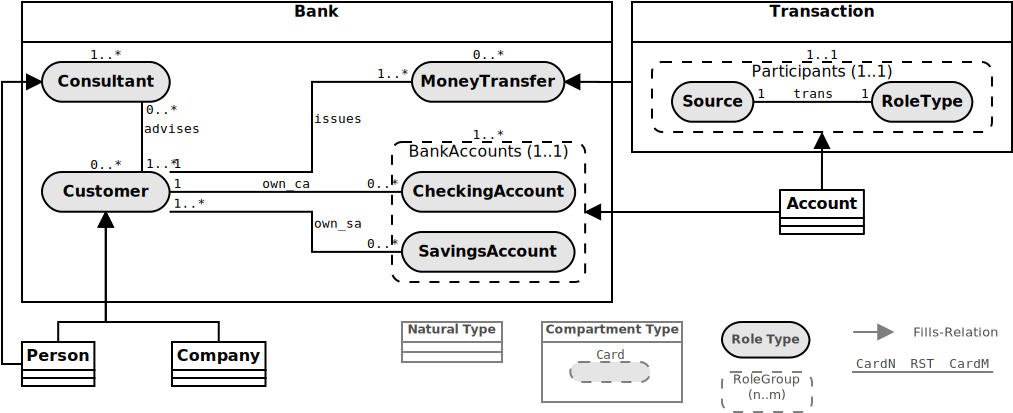
\includegraphics[width=\textwidth]{Bank-full-constraints}
  \BankFullConstraintsExample
  \caption{Graphical notation of a CROM for an banking application}
  \label{fig:bank}
\end{figure}

In our definitions, we omit to precisely define the graphical notation as they are not relevant for
reasoning on CROMs and refer to~\cite{KBG-SLE15}.

Next, we introduce instances of role-based models. An instance is based on a non-empty domain,
where each element is of exactly one type, i.e.\ a natural type, a \rosirole type or a compartment
type. Objects playing \rosirole in a compartment are collected in a ternary relation \plays and the
relation of two \rosiroles via a relationship type in a compartment is stored in \links.


\begin{definition}[Compartment Role Object Instance, Satisfiability]\label{def:scroi}
  Let $\Sigma = (\NT, \RT,$ $\CT,\RST)$ be a vocabulary.  Then, a
  \emph{Compartment Role Object Instance \I over $\Sigma$ (\SCROI)} is a tuple
  $\I=(\Gamma^{\I},\type,\plays,\links)$, where
  \begin{itemize}
  \item $\Gamma^{\I}$ is a non-empty domain, and
  \item $\type:\Gamma^{\I}\to\NT\cup\RT\cup\CT$ is a total function.
  \end{itemize}
  Based on the \type-function, we can partition the domain into the set \Nsf of \emph{naturals},
  i.e.\ all instances of any natural type, the set \Rsf of \emph{\rosiroles}, i.e.\ all instances of
  any \rosirole type, and the set \Csf of \emph{compartments}, i.e.\ all instances of any
  compartment type. Furthermore, the set \Osf of \emph{objects} denote all domain elements that are
  eligible to play a \rosirole, i.e.\ all naturals and compartments.
  \begin{align*}
    \Nsf & \coloneqq \{d \in \Gamma^{\I} \mid \type(d) \in \NT\} \\
    \Rsf & \coloneqq \{d \in \Gamma^{\I} \mid \type(d) \in \RT\} \\
    \Csf & \coloneqq \{d \in \Gamma^{\I} \mid \type(d) \in \CT\} \\
    \Osf & \coloneqq \Nsf \cup \Csf
  \end{align*}
  %
  Now, \plays and \links are defined as follows:
  \begin{itemize}
  \item $\plays \subseteq \Osf\times\Csf\times\Rsf$ is a ternary relation, and
  \item $\links: (\RST\times\Csf) \to \powerset{\Rsf\times\Rsf}$ is a total function.
  \end{itemize}
  %
  Furthermore, %
  the set $T^{\I}$ of all elements of type $T\in(\NT\cup\RT\cup\CT)$, %
  the set \Osf[\I,c] of all objects playing a role in $c$, %
  the set \Osf[\I,c,\rt] of all objects playing an \rt-role in $c$, and %
  the set \Rsf[\I,c] of all roles played in $c$ %
  are defined as follows:
  \begin{align*}
    T^{\I}     & \coloneqq \{d \in \Gamma \mid \type(d) = T\},\\
    \Osf[\I,c] & \coloneqq \{o \in \Osf \mid \text{there is some $r$ with $(o,c,r) \in \plays$}\}, \text{ and}\\
    \Osf[\I,c,\rt] & \coloneqq \{o \in \Osf \mid \text{there is some $r$ with $(o,c,r) \in \plays$
                     and $r\in\rt^{\I}$}\}\\
    \Rsf[\I,c] & \coloneqq \{r \in \Rsf \mid \text{there is some $o$ with $(o,c,r) \in \plays$}\}.
  \end{align*}
  %
  A \SCROI{} \I \emph{satisfies} a \SCROM{} \Mmc, denoted by $\I\models\Mmc$, if it has the following
  properties:
  \begin{enumerate}
  \item The \plays-relation respects \fills, i.e.~for each tuple $(o,c,r)\in\plays$ the type of $o$
    fills the type of $r$:
    \begin{align*}
      \{(o,r)\mid(o,\cdot,r)\in\plays\}\ \subseteq\ \{(o,r)\mid\text{there exists
        $(T,\rt)\in\fills$ s.t. $o\in T^{\I}$, $r\in \rt^{\I}$}\}.
    \end{align*}
  \item The \plays-relation respects \parts, i.e.~for each tuple $(o,c,r)\in\plays$ the type of $r$
    participates in the type of $c$:
    \begin{align*}
      & \{(c,r)\mid(\cdot,c,r)\in\plays\}\\
      & \quad \subseteq\ \{(c,r)\mid \text{there exists $\ct \in \CT$, $\rt \in \RT$ s.t. $c \in
        \ct^{\I}$, $r \in \rt^{\I}$, $\rt \in \parts(\ct)$}\}.
    \end{align*}
  \item Each object can only play one role of each role type in each compartment:
    \begin{align*}
      \{(o,c,r),(o,c,r')\}\subseteq\plays \textImplies \type(r)\neq\type(r').
    \end{align*}
  \item Each role is played by exactly one object in exactly one compartment:
    \begin{align*}
      |\{(o,c)\mid(o,c,r)\in\plays\}| = 1 \quad\text{for all $r \in \Rsf$}.
    \end{align*}
  \item Roles occurring in the image of \links are played in the associated compartment, i.e.\ for
    each $(r_{1},r_{2})\in\links(\rst,c)$ there exists objects that play $r_{1}$ and $r_{2}$ in $c$:
    \begin{align*}
      \{r_{1} \mid (r_{1},\cdot) \in \links(\cdot,c)\} \cup \{r_{2} \mid (\cdot,r_{2}) \in \links(\cdot,c)\} \ \subseteq\ \{r\mid(\cdot,c,r)\in\plays\}.
    \end{align*}
  \item The \links-function respects \rel, i.e.\ for each $(r_{1}, r_{2}) \in \links(\rst, \cdot)$ the
    types of $r_{1}$ and $r_{2}$ are related via \rst:
    \begin{align*}
      (r_{1},r_{2}) \in \links(\rst, \cdot) \textImplies \rel(\rst)=(\type(r_{1}),\type(r_{2})).
    \end{align*}
  \end{enumerate}

  A \SCROM{} \Mmc is \emph{satisfiable} if there exists any \SCROI{} \I such that $\I\models\Mmc$. 
\end{definition}

We say that $r$ is an $\rt$-role and $c$ is a $\ct$-compartment if, respectively,
$\type(r) = \rt \in \RT$ and $\type(c) = \ct \in \CT$.  Furthermore, \emph{$o$ plays $r$ in $c$} and
$o$ is the \emph{player} of $r$ if $(o,c,r) \in \plays$, and \emph{$r_{1}$ is linked to $r_{2}$ via
  $\rst$ in $c$} if $(r_{1}, r_{2}) \in \links(\rst, c)$.

% Again, it is easy to verify that our definition of a \SCROI satisfying a \SCROM is equivalent to the
% definition of~\cite{KBG-SLE15}.
% Since the \plays-relation respects the \fills- and the \parts-relation, if $o$ plays an \rt-role in
% a \ct-compartment, then the type of $o$ must fill \rt and \rt must participate in \ct. If $o$ plays
% $r_{1}$ and $r_{2}$ in $c$ then $r_{1}$ and $r_{2}$ must have different types, because each object
% can only play one role of each type in the same compartment. Moreover, for each role there exists
% exactly one object that plays it and one compartment where it is played in. In contrast to the
% formalisation in~\cite{KBG-SLE15} we omit $\varepsilon$-roles, but roles that are linked via a
% relationship type are both played in the same compartment and must be instances of the correct types
% since \links respects \rel.  Thus, equations (6) to (11) of~\cite{KBG-SLE15} are satisfied.

Before we investigate how the information about a \SCROM can be encoded in a description logic
ontology, we have to discuss the main reasoning tasks for role-based models. The arguably most
apparent question is, given a \SCROM{} \Mmc and a \SCROI{} \I, whether \I is compliant with
\Mmc. But as this task rather belongs to the area of model checking, we will not focus on that
problem in this thesis.
%
Instead, given a \SCROM{} \Mmc, it is more interesting whether there exists any \SCROI that is
compliant with \Mmc.  Additionally, we often want to know for a specific \SCROM{} \Mmc whether there
exists a compliant \SCROI that fulfills certain assertions, e.g.\ that a role of a certain type is
played.  To express this assertional knowledge, we introduce a so-called \SCROA, a finite set of
assertions which should additionally be satisfied by a \SCROI.

\begin{definition}[$\Sigma$-Compartment Role Object Assertions] \label{def:scroa} Let
  $\Sigma = (\NT, \RT, \CT, \RST)$ be a vocabulary and let \INDC and \IND be two non-empty, disjoint
  sets of meta and object individual names disjoint from $\Sigma$.  A \emph{Compartment Role Object
    Assertion over $\Sigma$} is of the form
  \begin{itemize}
  \item $T(c)$ with $T\in\CT$ and $c\in\INDC$ (\emph{meta type assertion}),
  \item $T(a,c)$ with $T \in \NT \cup \CT \cup \RT$, $a\in\IND$ and $c\in\INDC$ (\emph{object type assertion}),
  \item $\playass(a_{1}, c, a_{2})$ with $a_{1}, a_{2} \in \IND$ and $c\in\INDC$ (\emph{plays assertion}), or
  \item $\linkass(\rst, c, a_{1}, a_{2})$ with $\rst \in \RST$ and  $a_{1}, a_{2} \in \IND$ and
    $c\in\INDC$ (\emph{link assertion}). 
  \end{itemize}

  A \emph{set of Compartment Role Object Assertions \A over $\Sigma$ (\SCROA)} is a finite set of such
  assertions.
  %
  We extend the \SCROI{} \I to additionally map individual names to domain elements, e.g.\
  $a\in\IND$ and $c\in\INDC$ are
  mapped to a domain elements $a^{\I} \in \Gamma^{\I}$ and $c^{\I} \in \Gamma^{\I}$. A \SCROI{} \I \emph{satisfies an assertion
    $\alpha$}, denoted by $\I\models\alpha$, if the following conditions hold:
  \begin{itemize}
  \item if $\alpha = T(c)$, then $c^{\I} \in T^{\I}$,
  \item if $\alpha = T(a, c)$, then $a^{\I} \in T^{\I} \cap (\Osf\cup\Rsf[\I,c])$,
  \item if $\alpha = \playass(a_{1}, c, a_{2}, )$, then
    $(a_{1}^{\I}, c^{\I}, a_{2}^{\I}) \in \plays$, and
  \item if $\alpha = \linkass(\rst, c, a_{1}, a_{2})$, then there exist $r_{1}, r_{2} \in \Rsf$ with
    $(a_{1}, c, r_{1})\in\plays$, $(a_{2}, c, r_{2})\in\plays$ and
    $(r_{1}^{\I}, r_{2}^{\I}) \in \links(\rst, c^{\I})$.
  \end{itemize}

  A \SCROI{} \I \emph{satisfies \A}, denoted by $\I\models\A$ if it satisfies all assertions
  in \A.
\end{definition}

Note here that the link assertion asserts for two objects that they play roles which are related via
\rst, and not that the objects themselves are related.
%
Moreover, without any assertions there always exists a trivial CROI that satisfies \Mmc with the
singleton set $\Gamma = \{o\}$ where the type of $o$ is some natural type, and \plays and \links are
empty sets. Therefore, we introduce in the next section further constraints.


\subsubsection{Constraint Level}
\label{sec:constraint-level}

When modelling a domain of interest, not only the type of an object defines whether that object is
allowed to play a certain role. In~\cite{KBG-SLE15} additional constraints were introduced. These
can be divided into four groups.

\emph{Role constraints} are the first category of constraints which state, for example, that roles
mutually exclude each other or playing one role implies playing another role. More general these
constraints are formalised with so-called \emph{role groups}. These consist of a set of role types
(or again role groups), a lower and an upper bound. An object fulfills a role group if it plays at
least the lower and at most the upper bound of roles from the set of role types.

\begin{definition}[Syntax of role groups]\label{def:syntax-role-groups}
  Let \RT be a set of role types. The set of \emph{role groups over \RT} is the smallest such that
  \begin{itemize}
  \item if $\rt \in \RT$, then \rt is an (\emph{atomic}) role group, and
  \item if $A_{1}$, \dots, $A_{n}$ are role groups, $k,\ell \in \nat$, then $(\{A_{1}, \dots, A_{n}\},
    k,\ell)$ is a (\emph{complex}) role group.
  \end{itemize}
  \emph{Atoms} of a role group $A$ are defined as:
  \begin{align*}
    \atom(A) & \coloneqq
               \begin{cases}
                 \{\rt\} & \text{if $A = \rt \in \RT$}\\
                 \bigcup_{i=1}^{n} \atom(A_{i}) & \text{if $A = (\{A_{1}, \dots, A_{n}\},k,\ell)$}.
               \end{cases}
  \end{align*}
  Role groups that occur within other role groups are called \emph{nested}.
\end{definition}

The semantics of a role group are based on a \SCROI and are locally evaluated for each domain
element and each compartment.  The interpretation function $\cdot^{\I,c,o}$ calculates recursively
whether an object fulfills the role group.

\begin{definition}[Semantics of role groups]\label{def:semantics-role-groups}
  Given a \SCROI{} \I, the semantics of a role group~$A$ is defined for an object $o \in \Osf$ in
  $c \in \Csf$ as follows:
  \begin{align*}
    A^{\I,c,o} & \coloneqq 
                 \begin{cases}
                   1 & \text{if $A = \rt\in\RT$ and $o$ plays an \rt-role in $c$, or} \\
                     & \text{if $A = (\{B_{1},\dots,B_{n}\},k,\ell)$ and $k \leq \sum_{i=1}^{n}
                     B_{i}^{\I,c,o} \leq \ell$, and}\\
                   0 & \text{otherwise.}
                 \end{cases}
  \end{align*}

  If $A^{\I,c,o} = 1$, we say that $o$ fulfills $A$ in $c$.
\end{definition}

\noindent
Basic role constraints, for example as defined in~\cite{RiGr-OOPLSLA98}, i.e.\ role implication,
role equivalence and role prohibition, can be expressed with role groups as well as much more
complex ones. In fact, any propositional formula can be emulated with role groups.

\begin{proposition}
  Let $\varphi$ be some propositional formula. Then, there exists a role group $A_{\varphi}$ such
  that $\varphi$ is satisfiable if and only if $A_{\varphi}$ can be fulfilled.
\end{proposition}
\begin{proof}
  We define $A_{\varphi}$ inductively as follows:
  
  \vspace{\topsep}
  \begin{tabular}{@{ if }l@{\quad then\quad }l}
    $\varphi = p$ & $A_{\varphi} \coloneqq \rt[p]$,\\
    $\varphi = \lnot \psi$ & $A_{\varphi} \coloneqq (\{A_{\psi}\}, 0, 0)$,\\
    $\varphi = \psi_{1}\land\psi_{2}$ & $A_{\varphi} \coloneqq (\{A_{\psi_{1}}, A_{\psi_{2}}\}, 2, 2)$, and\\
    $\varphi = \psi_{1}\lor\psi_{2}$ & $A_{\varphi} \coloneqq (\{A_{\psi_{1}}, A_{\psi_{2}}\}, 1, 2)$.
  \end{tabular}
  \vspace{\topsep}
  
  \noindent
  Next, we establish a 1-to-1-relation between a valuation $\rho$ for $\varphi$ and a
  $\Sigma$-CROI{} \I. For every propositional variable $P_{i}$ occurring in $\varphi$, we introduce
  a role type \rt[i] and assume that $o$ plays an \rt[i]-role iff $\rho(P_{i}) = \true$. By
  induction, it follows that $\rho(\varphi) = \true$ iff $o$ fulfills $A_{\varphi}$.
\end{proof}


The next category of constraints are \emph{occurrence constraints}. These state how often a role
type or role group must at least or at most be played in a compartment. Therefore, we introduce the
notion of a \emph{cardinality}, a pair $(k,\ell)\in\nat\times\natinf$ with $k\leq\ell$. We usually
denote cardinalities by $(k..\ell)$. Since role types are also atomic role groups, it suffices to
specify occurrence constraints for role groups.
%
Similar to multiplicities specified for associations in UML class diagrams, we specify
\emph{cardinality constraints} for relationship types. They express how often a role of certain type
must be related via a relationship type to some other role type.

Last but not least, the category of \emph{intra-relationship type constraints} imposes constraints on the
players of roles which are related via a relationship type. For example, stating that the
relationship type $\mathsf{isAncestorOf}$ between the role types $\mathsf{Parent}$ and
$\mathsf{Child}$ is transitive assures the existence of a respective link between a grandparent and
a grandchild. Note here, that the transitivity is evaluated over the players and not the roles
themselves.

\begin{definition}[Constraint set]
  Let $\Sigma = (\NT, \RT, \CT, \RST)$ be a vocabulary, let \RG be the set of role groups over \RT
  and let $\Card \coloneqq \nat \times \natinf$ be the set of cardinalities.  Then, a
  \emph{$\Sigma$-Compartment Role Object Constraint Set (\SCROC) \Cmc} is a tuple $\CC$ where
  \begin{itemize}[topsep=5pt]
  \item $\occur : \CT \to \powerset{\Card \times \RG}$,
  \item $\card : \RST \to \Card \times \Card$, and
  \item $\intra : \RST \to \powerset{\Emc}$ with \Emc being a set of functions of the form
    $e : \powerset{A\times B}\to \{\true, \false\}$ for arbitrary sets $A$, $B$.
  \end{itemize}
  are total functions.  The set of all non-nested role groups that appear in \occur is the set of
  \emph{top-level role groups \RG*}.
  %
  A \SCROC{} \Cmc is \emph{compliant} to a \SCROM if all atoms of a role group that is in the occurrence
  constraints of a compartment type participate in that compartment type. 
  %
  Before we define satisfiability, we introduce the following auxiliary functions:
  \begin{align*}
    \Succ(\rst,r,c) & \coloneqq \{r' \in \Rsf \mid (r,r') \in \links(\rst,c)\}, \\
    \Pred(\rst,r,c) & \coloneqq \{r' \in \Rsf \mid (r',r) \in \links(\rst,c)\}\text{, and} \\
    \links^{*}(\rst,c) & \coloneqq \{ (o_{1}, o_{2}) \mid (r_{1}, r_{2}) \in \links(\rst,c) \text{
                         and } (o_{1}, c, r_{1}), (o_{2}, c, r_{2}) \in \plays\}.
  \end{align*}
  %
  A \SCROI{} \I \emph{satisfies \Cmc}, denoted by $\I\models\Cmc$, if it has the following
  properties:
  \begin{enumerate}
  \item All occurrence constraints are respected, i.e.\ if $(k..\ell,A) \in \occur(\ct)$, then in
    every \ct-compartment there must exist at least~$k$ and at most~$\ell$ objects that fulfill role
    group~$A$:
    \begin{align*}
      ((k,\ell),A) \in \occur(\ct) \textImplies  \ct^{\I} \subseteq \left\{c \in \Csf \mmid k \leq \sum\nolimits_{o\in\Osf[\I,c]}
      A^{\I,c,o} \leq \ell \right\}
    \end{align*}
  \item All top-level \rosirole groups must be satisfied, i.e.\ if an object~$o$ plays an \rt-role and
    \rt is an atom of a top-level \rosirole group~A, then $o$ must fulfill~$A$:
    \begin{align*}
      & (o,c,r) \in \plays \text{, } r \in \rt^{\I} \text{ and } \rt \in \atom(A) \textImplies
      A^{\I,c,o} = 1\text{,} \\
      & \hspace{8cm} \text{for all $o \in \Osf$, $A \in \RG*$}.
    \end{align*}
  \item All cardinality constraints are respected, i.e.\ every \rosirole that is played in a
    compartment~$c$ and whose type is either the domain or the range of a relationship type~\rst
    with $\card(\rst) = (i..j, k..\ell)$ must have at least~$k$ and at most~$\ell$ \rst-successors
    in~$c$ or at least~$i$ and at most~$j$ \rst-predecessors in~$c$, respectively:
    \begin{align*}
      & (\cdot,c,r) \in \plays \text{, } r \in \rt[1]^{\I} \text{, } \rel(\rst) = (\rt[1], \cdot) \text{ and
        } \card(\rst)=(\cdot,k..\ell)\\
      & \qquad \textImplies k \leq | \Succ(\rst,r,c) | \leq \ell
    \end{align*}
    \begin{align*}
      & (\cdot,c,r) \in \plays \text{, } r \in \rt[2]^{\I} \text{, } \rel(\rst) = (\cdot, \rt[2]) \text{ and
        } \card(\rst)=(i..j,\cdot)\\
      & \qquad \textImplies i \leq | \Pred(\rst,r,c) | \leq j
    \end{align*}

  \item All intra-relationship type constraints are respected, i.e.\ every function $\fsf \in
    \intra(\rst)$, evaluated over the players of the roles related via \rst, must return \true:
    \begin{align*}
      & \fsf \in \intra(\rst) \textImplies \fsf(\links^{*}(\rst,c)) = \true \\
      & \qquad\text{for all $c$ in $\ct^{\I}$ s.t.\ \rst participates in \ct}.\qedhere
    \end{align*}
  \end{enumerate}
\end{definition}

The definition of satisfying a constraint model in~\cite{KBG-SLE15} is, neglecting
$\varepsilon$-roles, exactly reflected in the above definition. With constraints being formally
introduced, we can complete the CROM for the banking application of Example~\ref{ex:bank-crom} and Figure~\ref{fig:bank}.

\begin{example}
  We first define the complex \rosirole groups that occur in our example. The \rosirole group
  $\mathsf{Participants}$ in the context of an transaction ensures that a single account cannot be
  both the source and the target of an transaction. The \rosirole group $\mathsf{BankAccounts}$
  states the same for savings and checking accounts in the context of a bank. A single account
  cannot attain both \rosiroles simultaneously. 
  \begin{align*}
    \mathsf{Participants} & \coloneqq (\{\mathsf{Source}, \mathsf{Target}\},1,1)\\
    \mathsf{BankAccounts} & \coloneqq (\{\mathsf{SavingsAccount}, \mathsf{CheckingAccount}\},1,1)
  \end{align*}
  We next analyse the occurrence constraints. In our example a bank can only exists if it contains
  at least on consultant and one bank account. A transaction has exactly one source or
  target\footnote{Note here, that this small modelling error is made on purpose. We will discuss its
    logical implications later. Actually a transaction has exactly one source \emph{and} one target,
    and, hence, exactly two participants.}.
  \begin{align*}
    \occur(\mathsf{Bank}) & \coloneqq \{(1..\infty, \mathsf{Consultant}), (1..\infty, \mathsf{BankAccounts})\}\\
    \occur(\mathsf{Transaction}) & \coloneqq \{(1..1,\mathsf{Participants})\}
  \end{align*}
  For the appearing cardinality constraints we assume the following in the context of a bank. A
  consultant must advise at least one customer but not every customer necessarily needs a
  consultant. A customer does not need to have any bank account, but every bank account needs to
  have an owner. A checking account has exactly one owner, a savings account could have several. A
  money transfer is issued by exactly one customer and each customer issues at least one money
  transfer. In the context of a transaction, there is a one-to-one connection between source and
  target. 
  \begin{align*}
    \card(\mathsf{advises}) & \coloneqq (0..\infty,1..\infty)\\
    \card(\mathsf{own\_ca}) & \coloneqq (1..1,0..\infty)\\
    \card(\mathsf{own\_sa}) & \coloneqq (1..\infty,0..\infty)\\
    \card(\mathsf{issues}) & \coloneqq (1..1,1..\infty)\\
    \card(\mathsf{trans}) & \coloneqq (1..1,1..1)
  \end{align*}
  The intra-relationship type constraints are empty since we do not have such constraints in our
  example. 
\end{example}




At last we combine all parts of the role-based system into one \emph{constrained
  $\Sigma$-compartment Object Role Model}.

\begin{definition}[Constrained $\Sigma$-Compartment Role Object Model]
  \label{def:constrained-sigma-crom}
  Let $\Sigma = (\NT, \RT,$ $ \CT, \RST)$ be a vocabulary, let~\Mmc be a \SCROM, let~\Amc be a \SCROA
  and let~\Cmc be a \SCROC.
  %
  Then, a \emph{Constrained $\Sigma$-Compartment Role Object Model \SCCROM} is the tuple
  $\Kmc = (\Mmc, \Amc, \Cmc)$.

  The \emph{satisfiability problem} for \SCCROM{s} is the problem of deciding for a given \SCCROM{}
  $\Kmc = (\Mmc, \Amc, \Cmc)$ whether there exists a \SCROI that satisfies~\Mmc,~\Amc and~\Cmc.
\end{definition}





%%% Local Variables:
%%% mode: latex
%%% TeX-master: "../thesis"
%%% End:
